\section{Experimental Design}
\label{sec:design}

\subsection{Datasets}
\label{sec:datasets}
The evaluation uses 40 Sentinel-2 L2A \SI{10}{m} regions, ten in each of
four land-cover classes (urban, water, forest, agriculture), from
$43.5^\circ$S to $64.1^\circ$N (Fig.~\ref{fig:region_map}; the per-region
list, with product identifiers and window sizes, is in the code and data
repository, \repourl). The sites are those of the companion study of
PSF-aware resampling onto HEALPix~\cite{delouis2026resample}, whose
$256\times256$-pixel patches are archived under a public dataset DOI. A
level-20 \term{carrier} tile needs a much larger native window. Each region is
therefore re-extracted here at the same anchor and, wherever the archive
still serves it, from the same product: one L2A B04 window of about
\SI{11}{km} ($\approx1100$ native pixels, the exact width recorded per
region). The two studies thus share sites, acquisitions and radiometric
conventions.

The native window is centred on the HEALPix tile that contains the
anchor, whose bounding box is \SI{9.0}{km} across. An anchor-centred
window would have to be twice as large, more than one granule reliably
covers near its edge; a tile-centred one needs the bounding box plus a
resampling halo, about \SI{11}{km}. No image content enters this choice.
A region is admitted only if a complete level-10 parent tile lies inside
its window with halo, if the native pixels under the footprint are
valid, and if the \term{equal-area UTM square} is complete. When invalid pixels
exceed $0.1\%$ of the footprint the region is rejected. Below that,
isolated invalid pixels are removed from the triangulation on the
HEALPix side and interpolated from finite neighbours on the UTM side,
symmetrically, and the per-region counts are reported with the data. The red band (B04) is then resampled
once onto the level-20 tile by Clough--Tocher interpolation
(Section~\ref{sec:resampler}), and the native B04 raster is cropped to the
\term{equal-area square} of Section~\ref{sec:utm_crop}.

\begin{figure}[t]
\centering
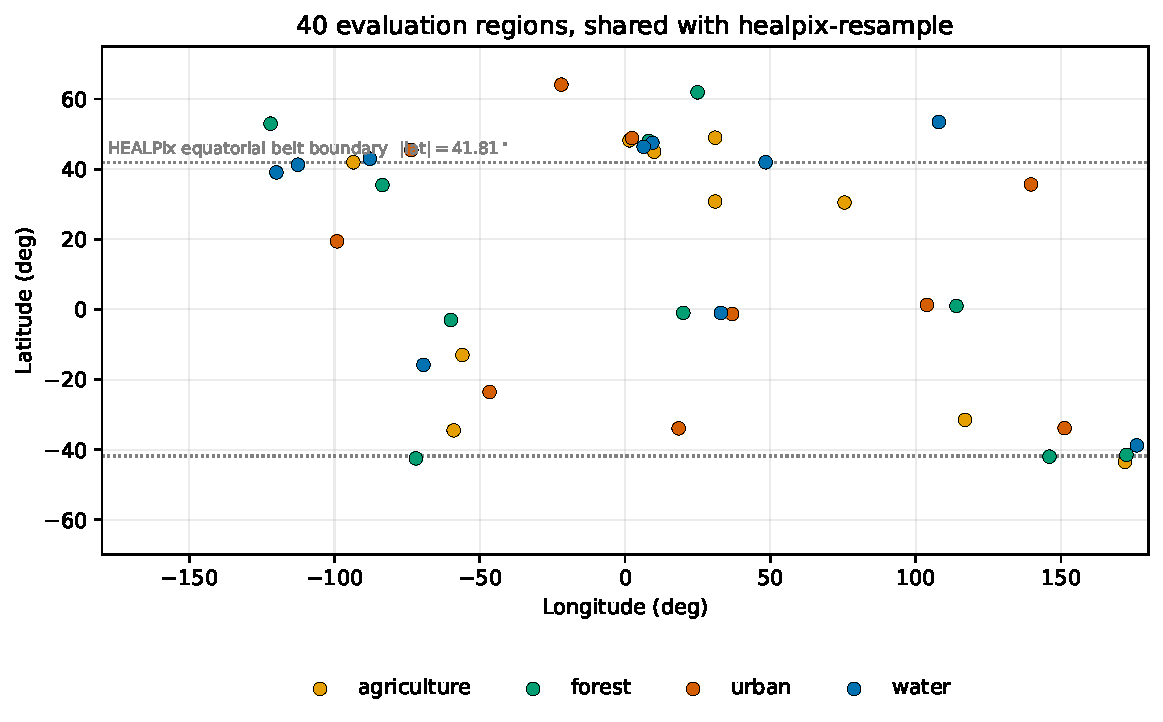
\includegraphics[width=\columnwidth]{figures/fig_region_map}
\caption{The 40 evaluation regions. Dotted lines mark $|\mathrm{lat}|=41.81^\circ$, the boundary between the equatorial belt and the polar caps of HEALPix, where the local cell-shape anisotropy changes character; both regimes are populated (22 and 18 regions).}
\label{fig:region_map}
\end{figure}

\subsection{Rate--Distortion Protocol}
\label{sec:rd_protocol}
Lossy codecs cannot be compared at a nominal setting. A quality level of
JPEG~2000, a tolerance of ZFP and an error bound of SZ3 mean different
things, and the same setting gives a different error on every
scene~\cite{lindstrom2014zfp,liang2022sz3}. Each codec is therefore swept
over its own parameter, and the resulting rate--distortion curves are
compared in one of two ways only: at the same reconstruction error,
compare sizes; or at the same size, compare errors. The two grids are
compared in the same way. A HEALPix tile and a \term{native square} are never
compared at the same codec setting; they are compared at the same
achieved error or the same budget. Every ratio in this paper is
therefore relative to a matched operating point, and none is an absolute
compression ratio.

For every (scene, codec, parameter) combination we record the encoded byte
count and the reconstruction RMSE against the raw tile (level-20 \term{carrier}
or \term{native crop}). The comparison at an \emph{achieved} error or size is
made by interpolating $\log(\text{size})$ against $\log(\text{RMSE})$,
and the inverse, on the sorted and de-duplicated sweep points.
Interpolating through a dominated configuration could in principle
produce a \term{target} no real configuration achieves. The analysis was
therefore repeated with each of the 400 (region, codec) sweeps
restricted to its Pareto frontier. This removes 44 dominated points,
almost all at the coarse end of the extended ladders, and changes no
reported median; at the $10^{-3}$ \term{target} it admits one more region and
moves the adjusted $p$-value from $0.016$ to $0.010$.

Three rules govern the \term{targets}. First, the curve is the constrained
problem $R(D)=\min\{S(q): d(q)\le D\}$: when a codec's coarsest setting is
already more accurate than the \term{target}, its size is a bound on what the
codec could achieve. Second, a (region, \term{target}) pair enters the paired
comparison only when the codec the oracle selects brackets the \term{target}
with two measured points on both grids, so that every ratio tested is an
interpolated estimate. A censored codec can be the smallest admissible
one, so this is stricter than asking some codec to bracket the \term{target}.
Every ladder was therefore extended at its coarse end
(Appendix~\ref{app:censoring}) until the only failing pairs were the
lowest-contrast scenes, where the \term{target} is a large fraction of the
scene's standard deviation or exceeds it. At $10^{-2}$ the eight
excluded regions are exactly those whose standard deviation is at most
$1.22$ times the \term{target} (six lakes and two smooth forests), and every
included region has at least $1.36$ times it. At tighter \term{targets} the one
to three exclusions are the smoothest lakes. A constant fill already
meets such a \term{target}, so the comparison is void there. Excluded pairs are counted, never
bounded; the $n$ of every table is the number that remain. Third, a
\term{target} for which fewer than $75\%$ of the regions qualify is withheld; the
$40\%$ and $20\%$ budgets ($0\%$ and $65\%$) fall under this rule. Every
reported \term{target} rests on 32 to 40 regions, and Appendix~\ref{app:censoring}
shows how each verdict would change if censored pairs were kept as bounds.
No extrapolation beyond a codec's measured range is performed.

\term{Target RMSE} values run from $10^{-4}$ to $10^{-2}$ (normalised
reflectance). Storage budgets run from $2\%$ to $40\%$ of one shared
reference, the raw size of the HEALPix tile (\num{4194304}~B), for both
grids; the UTM side receives this budget divided by $\gamma_{\mathrm{tile}}$
when an operational overhead is assumed (Section~\ref{sec:overhead}).
Codecs with a single operating point (the two lossless variants) are
reported at their achieved point only. All reported values are medians over
the regions that qualify. Every confidence interval on a median ratio is a
$95\%$ percentile bootstrap: the qualifying regions are resampled with
replacement $10\,000$ times, the median is recomputed on each resample,
and the interval runs from the $2.5$th to the $97.5$th percentile of
those medians. Paired $p$-values are two-sided Wilcoxon signed-rank
tests~\cite{wilcoxon1945} on the log ratios.

The \term{targets} should be read against the error the \term{transfer}
itself leaves, which is how the companion study sets the acceptable
reconstruction error on synthetic scenes~\cite{delouis2026resample}.
Appendix~\ref{app:error_budget} measures that error here on synthetic
fields built with each region's own spectrum, instrument response and
noise level. For the Clough--Tocher tile, scored against the observed
field it reproduces, the median error is $3.0\times10^{-3}$. The
tightest \term{target} is $3\%$ of it, the $3\times10^{-3}$
\term{target} is $1.0$ times it and the loosest is $3.4$ times it: the
three tightest \term{targets} compress well below the resampling error,
the fourth at its level and the loosest above it. For the PSF-aware
tile, scored against the latent field it estimates, the error is set by
the blur it does not remove: by class median, $2.8\times10^{-3}$ over
forest to $4.0\times10^{-2}$ over urban scenes. The companion study
reports that this \term{transfer} recovers $15.4\%$ to $19.6\%$ of that
blur on noise-free fields, and Appendix~\ref{app:error_budget} finds the
same range here at the nominal response width. An orthogonal
compression error of $1.5\times10^{-3}$ (forest) to $2.2\times10^{-2}$
(urban) would cancel the smaller of those recoveries, so on the
PSF-aware tile only the \term{targets} up to $10^{-3}$ preserve, in
every class, what the \term{transfer} restores.
Appendix~\ref{app:error_budget} carries the same accounting to the
crossings of Section~\ref{sec:results}.

\subsection{Operational UTM Storage}
\label{sec:overhead}
Sentinel-2 and comparable products are distributed as fixed geographic
tiles (MGRS granules with overlap bands), whose padding, overlap and
per-tile metadata add storage beyond the area needed. This overhead
belongs to the product organisation: UTM as a coordinate reference system
carries none of it, and a native UTM COG or Zarr archive need not either.
The tiling geometry constrains it from both sides. Sentinel-2 granules
are nominally \SI{110}{km} squares laid on a \SI{100}{km}
step~\cite{esa_s2_products}; a \SI{10}{m} band holds $10980$ pixels per
side, \SI{109.8}{km}, so the archive stores a fully covered area
$(109.8/100)^2=1.21$ times. That is a duplication of sample area, real
pixels held twice. What it costs in \emph{compressed} bytes is not
measured here. The duplicated bands are ordinary image content, but a
codec encodes each tile independently and the duplicate is coded in its
own context, so the byte overhead need not equal the area overhead. The
swath gives the raw figure. Across track, $3.998$ tiles on average over
the position of the swath edge store $3.998\times\SI{109.8}{km}$ of
raster for a \SI{290}{km} swath, a factor of $1.51$, of which $34\%$ is
no-data. Along track the overlap alone gives $1.098$. The product, $1.66$,
is the raw-byte overhead of the tiled swath. No-data compresses to
almost nothing, so under compression the figure falls back towards the
area duplication. A survey of the whole Sentinel-2 grid reaches the same
order: over the land surface, zone overlap and the enlarged granules
together store $33\%$ more area than the land covered ($13\%$ for the
zone overlap alone), which inflates the yearly Level-1C and Level-2A
volume by about one petabyte~\cite{bauer2023wasting}. That figure is
also a duplication of area, not a count of compressed bytes. We use
$\gamma_{\mathrm{tile}}=1.30$ as an illustrative point on the decision
curve of Section~\ref{sec:rd_main}. It lies between the geometric
sample-area duplication factor of $1.21$ and the raw tiled-swath factor
of $1.66$, at the level of the published spatial overhead. It is never a
measurement of a complete product file
(Section~\ref{sec:limitations}). $\gamma_{\mathrm{tile}}=1$ is the
overhead-free result.

For \emph{uncompressed} storage (Table~\ref{tab:storage_accounting}),
$\gamma_{\mathrm{tile}}$ multiplies the raw equal-area UTM byte count
once. For \emph{compressed} storage, applying it to the raw size alone
would assume that the padded $30\%$ of native pixels compresses to zero
bytes, which is unsafe for a codec that encodes each tile independently.
We therefore apply $\gamma_{\mathrm{tile}}$ to the \emph{compressed} byte
count of the \term{equal-area crop} and compare absolute bytes, with the raw size
of the fixed HEALPix tile ($\num{4194304}$ bytes) as the single reference
for both grids. The survey of~\cite{bauer2023wasting} supports the
order of magnitude of the \emph{spatial} overhead of the operational
grid; applying that multiplier to compressed bytes is an explicit
assumption of the decision model, not a measurement, which is why the
critical-overhead curve of Section~\ref{sec:rd_main} is the general
result and $1.30$ one point on it. The tile and the crop have different
pixel counts ($1024\times1024$ against $637\times637$), so only absolute
bytes for the same nominal area are comparable. For a budget given as a share of the
reference, the \term{UTM crop} receives the budget divided by
$\gamma_{\mathrm{tile}}$; the rest is taken by the operational padding.

The two rasters also differ in divisibility: a power of two against an
odd side that block and wavelet codecs must pad. Compressing each raster
against its own central sub-blocks shows no penalty for the odd side. Per
pixel, the $637^2$ crop costs $0.6\%$ less than the same reduction costs
the HEALPix raster, and padding the crop to $640^2$ changes its lossless
size by $0.2\%$. Larger rasters do cost less per pixel at loose \term{targets},
where a file's fixed cost weighs. The protocol compares whole files of
the same area, so that cost enters both sides alike.
